\documentclass[aspectratio=169, 12pt]{beamer}
\usepackage{ccicons}

% --- 极简核心设置 ---
\usetheme{default} 
\usecolortheme{dove} % 经典的黑白配色方案，没有任何杂色
\setbeamertemplate{navigation symbols}{} % 删掉右下角那些没用的微型图标
\setbeamertemplate{frametitle}[default][center] % 标题居中（如果喜欢左对齐就删掉center）

% --- 字体设置 (追求 LaTeX 原汁原味) ---
\usepackage[T1]{fontenc}
\usefonttheme{serif} % 强制使用衬线体，找回你的 Computer Modern 感

% --- 页面信息 ---
\title{\Huge Double Pendulum\\ and The Chaos Theory \vspace{-0.5em}}
\author[Winston]{Winston (Wenqin) Huang \vspace{-1em}}
\institute{Olive Tree International Academy \vspace{-1em}}
\date{\small May-June, 2026}

\begin{document}

% 封面页
\begin{frame}
    \titlepage
\end{frame}


% 左右分栏：学术 PPT 的标准姿态
%\begin{frame}{System Configuration}
%    \begin{columns}[c] % [c] 表示垂直居中对齐
%        
%        \column{.45\textwidth}
%        \textbf{Lagrangian Mechanics}
%        \vspace{0.3cm}
%        \begin{itemize}
%            \item Two degrees of freedom: $\theta_1, \theta_2$
%            \item High sensitivity to $t=0$
%            \item Non-linear coupling
%        \end{itemize}
%
%        \column{.5\textwidth}
%        % 这里放图，如果是本地文件就用 \includegraphics
%        \centering
%        \begin{exampleblock}{}
%            \[ \mathcal{L} = \frac{1}{2}(m_1+m_2)L_1^2\dot{\theta}_1^2 + \dots \]
%        \end{exampleblock}
%        \small \textit{Figure 1: Schematic of Double Pendulum}
%        
%    \end{columns}
%\end{frame}

\begin{frame}{Related CALCAB Knowledge}
    \vspace{-2em}
    \begin{description}
        \item[\textbf{Differential Equation}:]{It is the core of simulation algorithm we applied in this project, the entire simulation was run based on a differential equation derived by \textit{Lagrangian Mechanics}, so the differential equation we learned in unit 7 is the core of our project.}
        \item[\textbf{Limit and Approaching}:]{In our project, the observation of the simulation accuracy as time step changes is also a core part. By speculating the result approaches a value as step decreases (becomes more accurate), we could choose a suitable time step for simulation that is both efficient and accurate.}
    \end{description}
        
\end{frame}

\begin{frame}{Introduction To The Chaos Theory}
    \begin{columns}[c]
        \column{0.6\textwidth}
        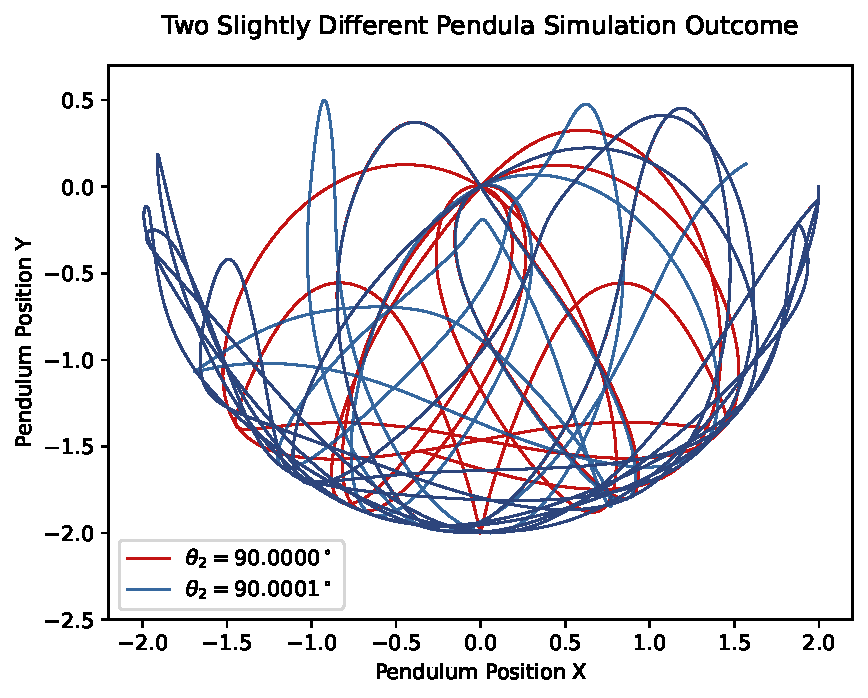
\includegraphics[width=\textwidth]{figures/Chaos_Intro.pdf}
        \\ \tiny Image by Winston Huang / CC BY 4.0 \ccby
        \column{0.45\textwidth}
         
        \small \textbf{Uncertain Outcome}: \small In a chaotic system described in the Chaos Theory, even a \textit{negligible} disturbance or initial differences could cause an incredibly different result.
        
        \small \textbf{Determinable though Chaotic}: \small Chaotic doesn't means random and indeterminate, instead, chaotic systems could be predicted by calculations and modeling if one have incredibly precise data, though the result is input-sensitive.

    \end{columns}
\end{frame}

\begin{frame}{Double Pendulum, Where Newtonian Physics Dies.}

\end{frame}

\begin{frame}{Introduction To DE Calculation Approaches}
    \begin{columns}[c]
        \column{0.5\textwidth}

        \column{0.45\textwidth}
        \textbf{\small Fourth-Order Runge-Kutta (RK4) Approach:}
        
    \end{columns} 
\end{frame}


\end{document}